\documentclass[1p]{elsarticle_modified}
%\bibliographystyle{elsarticle-num}

%\usepackage[colorlinks]{hyperref}
%\usepackage{abbrmath_seonhwa} %\Abb, \Ascr, \Acal ,\Abf, \Afrak
\usepackage{amsfonts}
\usepackage{amssymb}
\usepackage{amsmath}
\usepackage{amsthm}
\usepackage{scalefnt}
\usepackage{amsbsy}
\usepackage{kotex}
\usepackage{caption}
\usepackage{subfig}
\usepackage{color}
\usepackage{graphicx}
\usepackage{xcolor} %% white, black, red, green, blue, cyan, magenta, yellow
\usepackage{float}
\usepackage{setspace}
\usepackage{hyperref}

\usepackage{tikz}
\usetikzlibrary{arrows}

\usepackage{multirow}
\usepackage{array} % fixed length table
\usepackage{hhline}

%%%%%%%%%%%%%%%%%%%%%
\makeatletter
\renewcommand*\env@matrix[1][\arraystretch]{%
	\edef\arraystretch{#1}%
	\hskip -\arraycolsep
	\let\@ifnextchar\new@ifnextchar
	\array{*\c@MaxMatrixCols c}}
\makeatother %https://tex.stackexchange.com/questions/14071/how-can-i-increase-the-line-spacing-in-a-matrix
%%%%%%%%%%%%%%%

\usepackage[normalem]{ulem}

\newcommand{\msout}[1]{\ifmmode\text{\sout{\ensuremath{#1}}}\else\sout{#1}\fi}
%SOURCE: \msout is \stkout macro in https://tex.stackexchange.com/questions/20609/strikeout-in-math-mode

\newcommand{\cancel}[1]{
	\ifmmode
	{\color{red}\msout{#1}}
	\else
	{\color{red}\sout{#1}}
	\fi
}

\newcommand{\add}[1]{
	{\color{blue}\uwave{#1}}
}

\newcommand{\replace}[2]{
	\ifmmode
	{\color{red}\msout{#1}}{\color{blue}\uwave{#2}}
	\else
	{\color{red}\sout{#1}}{\color{blue}\uwave{#2}}
	\fi
}

\newcommand{\Sol}{\mathcal{S}} %segment
\newcommand{\D}{D} %diagram
\newcommand{\A}{\mathcal{A}} %arc


%%%%%%%%%%%%%%%%%%%%%%%%%%%%%5 test

\def\sl{\operatorname{\textup{SL}}(2,\Cbb)}
\def\psl{\operatorname{\textup{PSL}}(2,\Cbb)}
\def\quan{\mkern 1mu \triangleright \mkern 1mu}

\theoremstyle{definition}
\newtheorem{thm}{Theorem}[section]
\newtheorem{prop}[thm]{Proposition}
\newtheorem{lem}[thm]{Lemma}
\newtheorem{ques}[thm]{Question}
\newtheorem{cor}[thm]{Corollary}
\newtheorem{defn}[thm]{Definition}
\newtheorem{exam}[thm]{Example}
\newtheorem{rmk}[thm]{Remark}
\newtheorem{alg}[thm]{Algorithm}

\newcommand{\I}{\sqrt{-1}}
\begin{document}

%\begin{frontmatter}
%
%\title{Boundary parabolic representations of knots up to 8 crossings}
%
%%% Group authors per affiliation:
%\author{Yunhi Cho} 
%\address{Department of Mathematics, University of Seoul, Seoul, Korea}
%\ead{yhcho@uos.ac.kr}
%
%
%\author{Seonhwa Kim} %\fnref{s_kim}}
%\address{Center for Geometry and Physics, Institute for Basic Science, Pohang, 37673, Korea}
%\ead{ryeona17@ibs.re.kr}
%
%\author{Hyuk Kim}
%\address{Department of Mathematical Sciences, Seoul National University, Seoul 08826, Korea}
%\ead{hyukkim@snu.ac.kr}
%
%\author{Seokbeom Yoon}
%\address{Department of Mathematical Sciences, Seoul National University, Seoul, 08826,  Korea}
%\ead{sbyoon15@snu.ac.kr}
%
%\begin{abstract}
%We find all boundary parabolic representation of knots up to 8 crossings.
%
%\end{abstract}
%\begin{keyword}
%    \MSC[2010] 57M25 
%\end{keyword}
%
%\end{frontmatter}

%\linenumbers
%\tableofcontents
%
\newcommand\colored[1]{\textcolor{white}{\rule[-0.35ex]{0.8em}{1.4ex}}\kern-0.8em\color{red} #1}%
%\newcommand\colored[1]{\textcolor{white}{ #1}\kern-2.17ex	\textcolor{white}{ #1}\kern-1.81ex	\textcolor{white}{ #1}\kern-2.15ex\color{red}#1	}

{\Large $\underline{12n_{0668}~(K12n_{0668})}$}

\setlength{\tabcolsep}{10pt}
\renewcommand{\arraystretch}{1.6}
\vspace{1cm}\begin{tabular}{m{100pt}>{\centering\arraybackslash}m{274pt}}
\multirow{5}{120pt}{
	\centering
	\includegraphics[width=112pt]{../../../GIT/diagram.site/Diagrams/png/2757_12n_0668.png}\\
\ \ \ A knot diagram\footnotemark}&
\allowdisplaybreaks
\textbf{Linearized knot diagam} \\
\cline{2-2}
 &
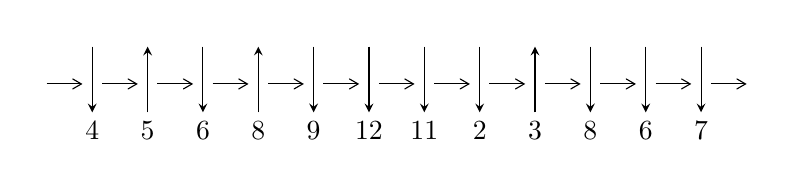
\begin{tikzpicture}[x=20pt, y=17pt]
	% nodes
	\node (C0) at (0, 0) {};
	\node (C1) at (1, 0) {};
	\node (C1U) at (1, +1) {};
	\node (C1D) at (1, -1) {4};

	\node (C2) at (2, 0) {};
	\node (C2U) at (2, +1) {};
	\node (C2D) at (2, -1) {5};

	\node (C3) at (3, 0) {};
	\node (C3U) at (3, +1) {};
	\node (C3D) at (3, -1) {6};

	\node (C4) at (4, 0) {};
	\node (C4U) at (4, +1) {};
	\node (C4D) at (4, -1) {8};

	\node (C5) at (5, 0) {};
	\node (C5U) at (5, +1) {};
	\node (C5D) at (5, -1) {9};

	\node (C6) at (6, 0) {};
	\node (C6U) at (6, +1) {};
	\node (C6D) at (6, -1) {12};

	\node (C7) at (7, 0) {};
	\node (C7U) at (7, +1) {};
	\node (C7D) at (7, -1) {11};

	\node (C8) at (8, 0) {};
	\node (C8U) at (8, +1) {};
	\node (C8D) at (8, -1) {2};

	\node (C9) at (9, 0) {};
	\node (C9U) at (9, +1) {};
	\node (C9D) at (9, -1) {3};

	\node (C10) at (10, 0) {};
	\node (C10U) at (10, +1) {};
	\node (C10D) at (10, -1) {8};

	\node (C11) at (11, 0) {};
	\node (C11U) at (11, +1) {};
	\node (C11D) at (11, -1) {6};

	\node (C12) at (12, 0) {};
	\node (C12U) at (12, +1) {};
	\node (C12D) at (12, -1) {7};
	\node (C13) at (13, 0) {};

	% arrows
	\draw[->,>={angle 60}]
	(C0) edge (C1) (C1) edge (C2) (C2) edge (C3) (C3) edge (C4) (C4) edge (C5) (C5) edge (C6) (C6) edge (C7) (C7) edge (C8) (C8) edge (C9) (C9) edge (C10) (C10) edge (C11) (C11) edge (C12) (C12) edge (C13) ;	\draw[->,>=stealth]
	(C1U) edge (C1D) (C2D) edge (C2U) (C3U) edge (C3D) (C4D) edge (C4U) (C5U) edge (C5D) (C6U) edge (C6D) (C7U) edge (C7D) (C8U) edge (C8D) (C9D) edge (C9U) (C10U) edge (C10D) (C11U) edge (C11D) (C12U) edge (C12D) ;
	\end{tikzpicture} \\
\hhline{~~} \\& 
\textbf{Solving Sequence} \\ \cline{2-2} 
 &
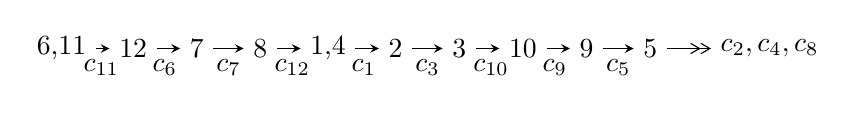
\begin{tikzpicture}[x=23pt, y=7pt]
	% node
	\node (A0) at (-1/8, 0) {6,11};
	\node (A1) at (1, 0) {12};
	\node (A2) at (2, 0) {7};
	\node (A3) at (3, 0) {8};
	\node (A4) at (65/16, 0) {1,4};
	\node (A5) at (41/8, 0) {2};
	\node (A6) at (49/8, 0) {3};
	\node (A7) at (57/8, 0) {10};
	\node (A8) at (65/8, 0) {9};
	\node (A9) at (73/8, 0) {5};
	\node (C1) at (1/2, -1) {$c_{11}$};
	\node (C2) at (3/2, -1) {$c_{6}$};
	\node (C3) at (5/2, -1) {$c_{7}$};
	\node (C4) at (7/2, -1) {$c_{12}$};
	\node (C5) at (37/8, -1) {$c_{1}$};
	\node (C6) at (45/8, -1) {$c_{3}$};
	\node (C7) at (53/8, -1) {$c_{10}$};
	\node (C8) at (61/8, -1) {$c_{9}$};
	\node (C9) at (69/8, -1) {$c_{5}$};
	\node (A10) at (11, 0) {$c_{2},c_{4},c_{8}$};

	% edge
	\draw[->,>=stealth]	
	(A0) edge (A1) (A1) edge (A2) (A2) edge (A3) (A3) edge (A4) (A4) edge (A5) (A5) edge (A6) (A6) edge (A7) (A7) edge (A8) (A8) edge (A9) ;
	\draw[->>,>={angle 60}]	
	(A9) edge (A10);
\end{tikzpicture} \\ 

\end{tabular} \\

\footnotetext{
The image of knot diagram is generated by the software ``\textbf{Draw programme}" developed by Andrew Bartholomew(\url{http://www.layer8.co.uk/maths/draw/index.htm\#Running-draw}), where we modified some parts for our purpose(\url{https://github.com/CATsTAILs/LinksPainter}).
}\phantom \\ \newline 
\centering \textbf{Ideals for irreducible components\footnotemark of $X_{\text{par}}$} 
 
\begin{align*}
I^u_{1}&=\langle 
-70612 u^{32}-259819 u^{31}+\cdots+11551 b+473521,\\
\phantom{I^u_{1}}&\phantom{= \langle  }70736 u^{32}+311623 u^{31}+\cdots+103959 a-759123,\;u^{33}+5 u^{32}+\cdots-27 u-9\rangle \\
I^u_{2}&=\langle 
- u^{15}+u^{14}+6 u^{13}-5 u^{12}-14 u^{11}+8 u^{10}+15 u^9-2 u^8-7 u^7-5 u^6+2 u^5+u^4+2 u^2+b-3 u+1,\\
\phantom{I^u_{2}}&\phantom{= \langle  }u^{15}- u^{14}-6 u^{13}+5 u^{12}+13 u^{11}-7 u^{10}-10 u^9- u^8-3 u^7+5 u^6+6 u^5+6 u^4+u^3-6 u^2+a- u-4,\\
\phantom{I^u_{2}}&\phantom{= \langle  }u^{16}-2 u^{15}-6 u^{14}+12 u^{13}+15 u^{12}-26 u^{11}-22 u^{10}+20 u^9+23 u^8+6 u^7-14 u^6-13 u^5-4 u^4+u^3+9 u^2+1\rangle \\
I^u_{3}&=\langle 
- u^{17} a-7 u^{17}+\cdots+a+7,\;- u^{17} a+u^{17}+\cdots- a+3,\;u^{18}-2 u^{17}+\cdots-2 u+1\rangle \\
I^u_{4}&=\langle 
b^2+b-1,\;a+1,\;u+1\rangle \\
\\
I^v_{1}&=\langle 
a,\;b+1,\;v-1\rangle \\
\end{align*}
\raggedright * 5 irreducible components of $\dim_{\mathbb{C}}=0$, with total 88 representations.\\
\footnotetext{All coefficients of polynomials are rational numbers. But the coefficients are sometimes approximated in decimal forms when there is not enough margin.}
\newpage
\renewcommand{\arraystretch}{1}
\centering \section*{I. $I^u_{1}= \langle -7.06\times10^{4} u^{32}-2.60\times10^{5} u^{31}+\cdots+1.16\times10^{4} b+4.74\times10^{5},\;7.07\times10^{4} u^{32}+3.12\times10^{5} u^{31}+\cdots+1.04\times10^{5} a-7.59\times10^{5},\;u^{33}+5 u^{32}+\cdots-27 u-9 \rangle$}
\flushleft \textbf{(i) Arc colorings}\\
\begin{tabular}{m{7pt} m{180pt} m{7pt} m{180pt} }
\flushright $a_{6}=$&$\begin{pmatrix}0\\u\end{pmatrix}$ \\
\flushright $a_{11}=$&$\begin{pmatrix}1\\0\end{pmatrix}$ \\
\flushright $a_{12}=$&$\begin{pmatrix}1\\u^2\end{pmatrix}$ \\
\flushright $a_{7}=$&$\begin{pmatrix}- u\\- u^3+u\end{pmatrix}$ \\
\flushright $a_{8}=$&$\begin{pmatrix}u^3-2 u\\- u^3+u\end{pmatrix}$ \\
\flushright $a_{1}=$&$\begin{pmatrix}- u^2+1\\- u^4+2 u^2\end{pmatrix}$ \\
\flushright $a_{4}=$&$\begin{pmatrix}-0.680422 u^{32}-2.99756 u^{31}+\cdots+13.8497 u+7.30214\\6.11306 u^{32}+22.4932 u^{31}+\cdots-91.7728 u-40.9939\end{pmatrix}$ \\
\flushright $a_{2}=$&$\begin{pmatrix}-11.9768 u^{32}-41.2941 u^{31}+\cdots+157.358 u+64.2446\\-3.85404 u^{32}-19.2469 u^{31}+\cdots+90.4188 u+47.0737\end{pmatrix}$ \\
\flushright $a_{3}=$&$\begin{pmatrix}-0.680422 u^{32}-2.99756 u^{31}+\cdots+13.8497 u+7.30214\\5.63986 u^{32}+22.1549 u^{31}+\cdots-96.5720 u-44.6349\end{pmatrix}$ \\
\flushright $a_{10}=$&$\begin{pmatrix}u^6-3 u^4+2 u^2+1\\- u^6+2 u^4- u^2\end{pmatrix}$ \\
\flushright $a_{9}=$&$\begin{pmatrix}0.537664 u^{32}+2.96977 u^{31}+\cdots-21.8762 u-9.12449\\-4.55935 u^{32}-18.5188 u^{31}+\cdots+82.5148 u+36.1951\end{pmatrix}$ \\
\flushright $a_{5}=$&$\begin{pmatrix}4.30313 u^{32}+14.8725 u^{31}+\cdots-56.2462 u-22.2317\\0.236603 u^{32}+3.16916 u^{31}+\cdots-20.1004 u-12.6795\end{pmatrix}$\\&\end{tabular}
\flushleft \textbf{(ii) Obstruction class $= -1$}\\~\\
\flushleft \textbf{(iii) Cusp Shapes $= -\frac{924167}{11551} u^{32}-\frac{3254604}{11551} u^{31}+\cdots+\frac{13356036}{11551} u+\frac{5544210}{11551}$}\\~\\
\newpage\renewcommand{\arraystretch}{1}
\flushleft \textbf{(iv) u-Polynomials at the component}\newline \\
\begin{tabular}{m{50pt}|m{274pt}}
Crossings & \hspace{64pt}u-Polynomials at each crossing \\
\hline $$\begin{aligned}c_{1},c_{3}\end{aligned}$$&$\begin{aligned}
&u^{33}+2 u^{32}+\cdots+7 u-1
\end{aligned}$\\
\hline $$\begin{aligned}c_{2}\end{aligned}$$&$\begin{aligned}
&u^{33}+22 u^{32}+\cdots+90 u+9
\end{aligned}$\\
\hline $$\begin{aligned}c_{4},c_{9}\end{aligned}$$&$\begin{aligned}
&u^{33}-2 u^{32}+\cdots-37 u+7
\end{aligned}$\\
\hline $$\begin{aligned}c_{5},c_{8}\end{aligned}$$&$\begin{aligned}
&u^{33}- u^{32}+\cdots+2 u+1
\end{aligned}$\\
\hline $$\begin{aligned}c_{6},c_{11},c_{12}\end{aligned}$$&$\begin{aligned}
&u^{33}+5 u^{32}+\cdots-27 u-9
\end{aligned}$\\
\hline $$\begin{aligned}c_{7},c_{10}\end{aligned}$$&$\begin{aligned}
&u^{33}-15 u^{32}+\cdots-621 u+1341
\end{aligned}$\\
\hline
\end{tabular}\\~\\
\newpage\renewcommand{\arraystretch}{1}
\flushleft \textbf{(v) Riley Polynomials at the component}\newline \\
\begin{tabular}{m{50pt}|m{274pt}}
Crossings & \hspace{64pt}Riley Polynomials at each crossing \\
\hline $$\begin{aligned}c_{1},c_{3}\end{aligned}$$&$\begin{aligned}
&y^{33}-50 y^{32}+\cdots+37 y-1
\end{aligned}$\\
\hline $$\begin{aligned}c_{2}\end{aligned}$$&$\begin{aligned}
&y^{33}+58 y^{31}+\cdots-540 y-81
\end{aligned}$\\
\hline $$\begin{aligned}c_{4},c_{9}\end{aligned}$$&$\begin{aligned}
&y^{33}+18 y^{32}+\cdots+1173 y-49
\end{aligned}$\\
\hline $$\begin{aligned}c_{5},c_{8}\end{aligned}$$&$\begin{aligned}
&y^{33}-13 y^{32}+\cdots+30 y-1
\end{aligned}$\\
\hline $$\begin{aligned}c_{6},c_{11},c_{12}\end{aligned}$$&$\begin{aligned}
&y^{33}-33 y^{32}+\cdots+351 y-81
\end{aligned}$\\
\hline $$\begin{aligned}c_{7},c_{10}\end{aligned}$$&$\begin{aligned}
&y^{33}-13 y^{32}+\cdots+28562733 y-1798281
\end{aligned}$\\
\hline
\end{tabular}\\~\\
\newpage\flushleft \textbf{(vi) Complex Volumes and Cusp Shapes}
$$\begin{array}{c|c|c}  
\text{Solutions to }I^u_{1}& \I (\text{vol} + \sqrt{-1}CS) & \text{Cusp shape}\\
 \hline 
\begin{aligned}
u &= \phantom{-}0.615295 + 0.690025 I \\
a &= -0.98614 + 1.55343 I \\
b &= -0.40560 - 1.50849 I\end{aligned}
 & -6.37902 + 7.26772 I & -8.48178 - 3.05803 I \\ \hline\begin{aligned}
u &= \phantom{-}0.615295 - 0.690025 I \\
a &= -0.98614 - 1.55343 I \\
b &= -0.40560 + 1.50849 I\end{aligned}
 & -6.37902 - 7.26772 I & -8.48178 + 3.05803 I \\ \hline\begin{aligned}
u &= \phantom{-}0.457629 + 0.777634 I \\
a &= -1.51279 + 1.36228 I \\
b &= \phantom{-}0.72143 - 1.81895 I\end{aligned}
 & -5.86299 - 12.19570 I & -7.30193 + 8.04387 I \\ \hline\begin{aligned}
u &= \phantom{-}0.457629 - 0.777634 I \\
a &= -1.51279 - 1.36228 I \\
b &= \phantom{-}0.72143 + 1.81895 I\end{aligned}
 & -5.86299 + 12.19570 I & -7.30193 - 8.04387 I \\ \hline\begin{aligned}
u &= -0.087307 + 0.812187 I \\
a &= -0.141714 + 0.501526 I \\
b &= \phantom{-}0.491481 - 0.424666 I\end{aligned}
 & \phantom{-}2.71643 + 3.62722 I & -8.53869 - 2.13399 I \\ \hline\begin{aligned}
u &= -0.087307 - 0.812187 I \\
a &= -0.141714 - 0.501526 I \\
b &= \phantom{-}0.491481 + 0.424666 I\end{aligned}
 & \phantom{-}2.71643 - 3.62722 I & -8.53869 + 2.13399 I \\ \hline\begin{aligned}
u &= -1.161150 + 0.326234 I \\
a &= \phantom{-}0.206831 - 0.059375 I \\
b &= -0.393012 - 0.608436 I\end{aligned}
 & -0.540380 + 0.517517 I & -9.25187 - 4.14256 I \\ \hline\begin{aligned}
u &= -1.161150 - 0.326234 I \\
a &= \phantom{-}0.206831 + 0.059375 I \\
b &= -0.393012 + 0.608436 I\end{aligned}
 & -0.540380 - 0.517517 I & -9.25187 + 4.14256 I \\ \hline\begin{aligned}
u &= \phantom{-}0.430358 + 0.659643 I \\
a &= \phantom{-}0.91402 - 1.98819 I \\
b &= -0.01529 + 1.61480 I\end{aligned}
 & -4.97909 - 0.59659 I & -11.69644 - 1.11532 I \\ \hline\begin{aligned}
u &= \phantom{-}0.430358 - 0.659643 I \\
a &= \phantom{-}0.91402 + 1.98819 I \\
b &= -0.01529 - 1.61480 I\end{aligned}
 & -4.97909 + 0.59659 I & -11.69644 + 1.11532 I\\
 \hline 
 \end{array}$$\newpage$$\begin{array}{c|c|c}  
\text{Solutions to }I^u_{1}& \I (\text{vol} + \sqrt{-1}CS) & \text{Cusp shape}\\
 \hline 
\begin{aligned}
u &= \phantom{-}0.478485 + 0.624833 I \\
a &= \phantom{-}1.95619 - 1.29179 I \\
b &= -0.69033 + 1.45431 I\end{aligned}
 & -5.15410 - 3.61074 I & -12.7241 + 8.1859 I \\ \hline\begin{aligned}
u &= \phantom{-}0.478485 - 0.624833 I \\
a &= \phantom{-}1.95619 + 1.29179 I \\
b &= -0.69033 - 1.45431 I\end{aligned}
 & -5.15410 + 3.61074 I & -12.7241 - 8.1859 I \\ \hline\begin{aligned}
u &= -1.23864\phantom{ +0.000000I} \\
a &= \phantom{-}0.294761\phantom{ +0.000000I} \\
b &= -1.07773\phantom{ +0.000000I}\end{aligned}
 & -2.25658\phantom{ +0.000000I} & -4.76340\phantom{ +0.000000I} \\ \hline\begin{aligned}
u &= \phantom{-}1.26064\phantom{ +0.000000I} \\
a &= \phantom{-}0.775692\phantom{ +0.000000I} \\
b &= \phantom{-}0.800176\phantom{ +0.000000I}\end{aligned}
 & -5.61796\phantom{ +0.000000I} & -16.2880\phantom{ +0.000000I} \\ \hline\begin{aligned}
u &= \phantom{-}1.347420 + 0.163931 I \\
a &= \phantom{-}0.321296 + 0.675196 I \\
b &= \phantom{-}0.111312 + 0.951165 I\end{aligned}
 & -4.31416 - 4.24029 I & \phantom{-0.000000 -}0. + 5.24975 I \\ \hline\begin{aligned}
u &= \phantom{-}1.347420 - 0.163931 I \\
a &= \phantom{-}0.321296 - 0.675196 I \\
b &= \phantom{-}0.111312 - 0.951165 I\end{aligned}
 & -4.31416 + 4.24029 I & \phantom{-0.000000 } 0. - 5.24975 I \\ \hline\begin{aligned}
u &= \phantom{-}1.307390 + 0.370979 I \\
a &= -0.395726 + 0.191298 I \\
b &= -0.565963 - 0.166815 I\end{aligned}
 & -1.64117 - 7.89167 I & \phantom{-0.000000 } 0 \\ \hline\begin{aligned}
u &= \phantom{-}1.307390 - 0.370979 I \\
a &= -0.395726 - 0.191298 I \\
b &= -0.565963 + 0.166815 I\end{aligned}
 & -1.64117 + 7.89167 I & \phantom{-0.000000 } 0 \\ \hline\begin{aligned}
u &= -1.39825\phantom{ +0.000000I} \\
a &= -1.11011\phantom{ +0.000000I} \\
b &= \phantom{-}1.72724\phantom{ +0.000000I}\end{aligned}
 & -6.43514\phantom{ +0.000000I} & -13.8800\phantom{ +0.000000I} \\ \hline\begin{aligned}
u &= -0.161042 + 0.523048 I \\
a &= -0.958016 + 0.069367 I \\
b &= \phantom{-}0.421774 + 0.647047 I\end{aligned}
 & \phantom{-}0.41915 + 1.76265 I & -3.15254 - 5.56900 I\\
 \hline 
 \end{array}$$\newpage$$\begin{array}{c|c|c}  
\text{Solutions to }I^u_{1}& \I (\text{vol} + \sqrt{-1}CS) & \text{Cusp shape}\\
 \hline 
\begin{aligned}
u &= -0.161042 - 0.523048 I \\
a &= -0.958016 - 0.069367 I \\
b &= \phantom{-}0.421774 - 0.647047 I\end{aligned}
 & \phantom{-}0.41915 - 1.76265 I & -3.15254 + 5.56900 I \\ \hline\begin{aligned}
u &= \phantom{-}1.46232 + 0.04987 I \\
a &= \phantom{-}0.207692 - 0.644243 I \\
b &= \phantom{-}0.408897 - 0.964739 I\end{aligned}
 & -7.32359 + 0.12289 I & \phantom{-0.000000 } 0 \\ \hline\begin{aligned}
u &= \phantom{-}1.46232 - 0.04987 I \\
a &= \phantom{-}0.207692 + 0.644243 I \\
b &= \phantom{-}0.408897 + 0.964739 I\end{aligned}
 & -7.32359 - 0.12289 I & \phantom{-0.000000 } 0 \\ \hline\begin{aligned}
u &= -1.47199 + 0.24653 I \\
a &= -1.246970 - 0.231738 I \\
b &= \phantom{-}0.32685 + 2.11863 I\end{aligned}
 & -11.11090 + 3.92371 I & \phantom{-0.000000 } 0 \\ \hline\begin{aligned}
u &= -1.47199 - 0.24653 I \\
a &= -1.246970 + 0.231738 I \\
b &= \phantom{-}0.32685 - 2.11863 I\end{aligned}
 & -11.11090 - 3.92371 I & \phantom{-0.000000 } 0 \\ \hline\begin{aligned}
u &= -0.494115 + 0.101505 I \\
a &= -0.444814 + 0.225779 I \\
b &= -0.395720 + 0.470268 I\end{aligned}
 & -1.070850 + 0.384320 I & -10.13714 - 2.26166 I \\ \hline\begin{aligned}
u &= -0.494115 - 0.101505 I \\
a &= -0.444814 - 0.225779 I \\
b &= -0.395720 - 0.470268 I\end{aligned}
 & -1.070850 - 0.384320 I & -10.13714 + 2.26166 I \\ \hline\begin{aligned}
u &= -1.48426 + 0.22127 I \\
a &= -1.39684 + 0.31844 I \\
b &= \phantom{-}1.23193 + 1.83135 I\end{aligned}
 & -11.50660 + 6.70613 I & \phantom{-0.000000 } 0 \\ \hline\begin{aligned}
u &= -1.48426 - 0.22127 I \\
a &= -1.39684 - 0.31844 I \\
b &= \phantom{-}1.23193 - 1.83135 I\end{aligned}
 & -11.50660 - 6.70613 I & \phantom{-0.000000 } 0 \\ \hline\begin{aligned}
u &= -1.50332 + 0.28479 I \\
a &= \phantom{-}1.319620 - 0.230307 I \\
b &= -0.82368 - 2.17854 I\end{aligned}
 & -12.2142 + 16.0764 I & \phantom{-0.000000 } 0\\
 \hline 
 \end{array}$$\newpage$$\begin{array}{c|c|c}  
\text{Solutions to }I^u_{1}& \I (\text{vol} + \sqrt{-1}CS) & \text{Cusp shape}\\
 \hline 
\begin{aligned}
u &= -1.50332 - 0.28479 I \\
a &= \phantom{-}1.319620 + 0.230307 I \\
b &= -0.82368 + 2.17854 I\end{aligned}
 & -12.2142 - 16.0764 I & \phantom{-0.000000 } 0 \\ \hline\begin{aligned}
u &= -1.54758 + 0.20289 I \\
a &= \phantom{-}1.177190 + 0.120725 I \\
b &= -0.14892 - 1.47002 I\end{aligned}
 & -13.53260 - 4.04812 I & \phantom{-0.000000 } 0 \\ \hline\begin{aligned}
u &= -1.54758 - 0.20289 I \\
a &= \phantom{-}1.177190 - 0.120725 I \\
b &= -0.14892 + 1.47002 I\end{aligned}
 & -13.53260 + 4.04812 I & \phantom{-0.000000 } 0\\
 \hline 
 \end{array}$$\newpage\newpage\renewcommand{\arraystretch}{1}
\centering \section*{II. $I^u_{2}= \langle - u^{15}+u^{14}+\cdots+b+1,\;u^{15}- u^{14}+\cdots+a-4,\;u^{16}-2 u^{15}+\cdots+9 u^2+1 \rangle$}
\flushleft \textbf{(i) Arc colorings}\\
\begin{tabular}{m{7pt} m{180pt} m{7pt} m{180pt} }
\flushright $a_{6}=$&$\begin{pmatrix}0\\u\end{pmatrix}$ \\
\flushright $a_{11}=$&$\begin{pmatrix}1\\0\end{pmatrix}$ \\
\flushright $a_{12}=$&$\begin{pmatrix}1\\u^2\end{pmatrix}$ \\
\flushright $a_{7}=$&$\begin{pmatrix}- u\\- u^3+u\end{pmatrix}$ \\
\flushright $a_{8}=$&$\begin{pmatrix}u^3-2 u\\- u^3+u\end{pmatrix}$ \\
\flushright $a_{1}=$&$\begin{pmatrix}- u^2+1\\- u^4+2 u^2\end{pmatrix}$ \\
\flushright $a_{4}=$&$\begin{pmatrix}- u^{15}+u^{14}+\cdots+u+4\\u^{15}- u^{14}+\cdots+3 u-1\end{pmatrix}$ \\
\flushright $a_{2}=$&$\begin{pmatrix}2 u^{15}-3 u^{14}+\cdots-4 u^2+10 u\\-3 u^{15}+2 u^{14}+\cdots- u+1\end{pmatrix}$ \\
\flushright $a_{3}=$&$\begin{pmatrix}- u^{15}+u^{14}+\cdots+u+4\\3 u^{15}-2 u^{14}+\cdots+2 u-2\end{pmatrix}$ \\
\flushright $a_{10}=$&$\begin{pmatrix}u^6-3 u^4+2 u^2+1\\- u^6+2 u^4- u^2\end{pmatrix}$ \\
\flushright $a_{9}=$&$\begin{pmatrix}- u^{14}+u^{13}+\cdots+7 u-1\\3 u^{15}-2 u^{14}+\cdots-5 u-3\end{pmatrix}$ \\
\flushright $a_{5}=$&$\begin{pmatrix}-2 u^{15}+2 u^{14}+\cdots+11 u^2+4\\3 u^{15}-2 u^{14}+\cdots+3 u-2\end{pmatrix}$\\&\end{tabular}
\flushleft \textbf{(ii) Obstruction class $= 1$}\\~\\
\flushleft \textbf{(iii) Cusp Shapes $= -6 u^{15}+u^{14}+40 u^{13}+7 u^{12}-101 u^{11}-62 u^{10}+95 u^9+144 u^8+34 u^7-109 u^6-111 u^5-33 u^4+29 u^3+52 u^2+22 u+5$}\\~\\
\newpage\renewcommand{\arraystretch}{1}
\flushleft \textbf{(iv) u-Polynomials at the component}\newline \\
\begin{tabular}{m{50pt}|m{274pt}}
Crossings & \hspace{64pt}u-Polynomials at each crossing \\
\hline $$\begin{aligned}c_{1},c_{3}\end{aligned}$$&$\begin{aligned}
&u^{16}-7 u^{15}+\cdots-4 u+1
\end{aligned}$\\
\hline $$\begin{aligned}c_{2}\end{aligned}$$&$\begin{aligned}
&u^{16}+9 u^{15}+\cdots+11 u+5
\end{aligned}$\\
\hline $$\begin{aligned}c_{4},c_{9}\end{aligned}$$&$\begin{aligned}
&u^{16}- u^{15}+\cdots+2 u^2+1
\end{aligned}$\\
\hline $$\begin{aligned}c_{5},c_{8}\end{aligned}$$&$\begin{aligned}
&u^{16}+2 u^{14}+\cdots+u+1
\end{aligned}$\\
\hline $$\begin{aligned}c_{6}\end{aligned}$$&$\begin{aligned}
&u^{16}+2 u^{15}+\cdots+9 u^2+1
\end{aligned}$\\
\hline $$\begin{aligned}c_{7}\end{aligned}$$&$\begin{aligned}
&u^{16}-6 u^{15}+\cdots-12 u+5
\end{aligned}$\\
\hline $$\begin{aligned}c_{10}\end{aligned}$$&$\begin{aligned}
&u^{16}+6 u^{15}+\cdots+12 u+5
\end{aligned}$\\
\hline $$\begin{aligned}c_{11},c_{12}\end{aligned}$$&$\begin{aligned}
&u^{16}-2 u^{15}+\cdots+9 u^2+1
\end{aligned}$\\
\hline
\end{tabular}\\~\\
\newpage\renewcommand{\arraystretch}{1}
\flushleft \textbf{(v) Riley Polynomials at the component}\newline \\
\begin{tabular}{m{50pt}|m{274pt}}
Crossings & \hspace{64pt}Riley Polynomials at each crossing \\
\hline $$\begin{aligned}c_{1},c_{3}\end{aligned}$$&$\begin{aligned}
&y^{16}- y^{15}+\cdots+16 y+1
\end{aligned}$\\
\hline $$\begin{aligned}c_{2}\end{aligned}$$&$\begin{aligned}
&y^{16}-3 y^{15}+\cdots-191 y+25
\end{aligned}$\\
\hline $$\begin{aligned}c_{4},c_{9}\end{aligned}$$&$\begin{aligned}
&y^{16}+7 y^{15}+\cdots+4 y+1
\end{aligned}$\\
\hline $$\begin{aligned}c_{5},c_{8}\end{aligned}$$&$\begin{aligned}
&y^{16}+4 y^{15}+\cdots+7 y+1
\end{aligned}$\\
\hline $$\begin{aligned}c_{6},c_{11},c_{12}\end{aligned}$$&$\begin{aligned}
&y^{16}-16 y^{15}+\cdots+18 y+1
\end{aligned}$\\
\hline $$\begin{aligned}c_{7},c_{10}\end{aligned}$$&$\begin{aligned}
&y^{16}+18 y^{14}+\cdots+396 y+25
\end{aligned}$\\
\hline
\end{tabular}\\~\\
\newpage\flushleft \textbf{(vi) Complex Volumes and Cusp Shapes}
$$\begin{array}{c|c|c}  
\text{Solutions to }I^u_{2}& \I (\text{vol} + \sqrt{-1}CS) & \text{Cusp shape}\\
 \hline 
\begin{aligned}
u &= -0.513943 + 0.697356 I \\
a &= -1.22872 - 1.28747 I \\
b &= \phantom{-}0.23245 + 1.44429 I\end{aligned}
 & -4.25844 + 2.34152 I & -8.19461 - 3.09667 I \\ \hline\begin{aligned}
u &= -0.513943 - 0.697356 I \\
a &= -1.22872 + 1.28747 I \\
b &= \phantom{-}0.23245 - 1.44429 I\end{aligned}
 & -4.25844 - 2.34152 I & -8.19461 + 3.09667 I \\ \hline\begin{aligned}
u &= -0.041928 + 0.737611 I \\
a &= -0.828729 - 0.160875 I \\
b &= \phantom{-}0.811180 - 0.178567 I\end{aligned}
 & \phantom{-}3.49750 + 3.94912 I & \phantom{-}1.82875 - 5.70898 I \\ \hline\begin{aligned}
u &= -0.041928 - 0.737611 I \\
a &= -0.828729 + 0.160875 I \\
b &= \phantom{-}0.811180 + 0.178567 I\end{aligned}
 & \phantom{-}3.49750 - 3.94912 I & \phantom{-}1.82875 + 5.70898 I \\ \hline\begin{aligned}
u &= -1.239030 + 0.314632 I \\
a &= -0.137190 - 0.504551 I \\
b &= -0.482263 - 0.342547 I\end{aligned}
 & -0.197771 - 0.146116 I & -3.97287 + 4.66079 I \\ \hline\begin{aligned}
u &= -1.239030 - 0.314632 I \\
a &= -0.137190 + 0.504551 I \\
b &= -0.482263 + 0.342547 I\end{aligned}
 & -0.197771 + 0.146116 I & -3.97287 - 4.66079 I \\ \hline\begin{aligned}
u &= \phantom{-}1.331470 + 0.116092 I \\
a &= -0.300310 - 0.649478 I \\
b &= \phantom{-}1.39100 + 0.87664 I\end{aligned}
 & -3.21145 + 2.06263 I & -9.83386 - 3.81751 I \\ \hline\begin{aligned}
u &= \phantom{-}1.331470 - 0.116092 I \\
a &= -0.300310 + 0.649478 I \\
b &= \phantom{-}1.39100 - 0.87664 I\end{aligned}
 & -3.21145 - 2.06263 I & -9.83386 + 3.81751 I \\ \hline\begin{aligned}
u &= \phantom{-}1.306250 + 0.303862 I \\
a &= \phantom{-}0.116790 + 0.407149 I \\
b &= -1.108390 - 0.136579 I\end{aligned}
 & -0.72717 - 7.70203 I & -3.85260 + 5.91558 I \\ \hline\begin{aligned}
u &= \phantom{-}1.306250 - 0.303862 I \\
a &= \phantom{-}0.116790 - 0.407149 I \\
b &= -1.108390 + 0.136579 I\end{aligned}
 & -0.72717 + 7.70203 I & -3.85260 - 5.91558 I\\
 \hline 
 \end{array}$$\newpage$$\begin{array}{c|c|c}  
\text{Solutions to }I^u_{2}& \I (\text{vol} + \sqrt{-1}CS) & \text{Cusp shape}\\
 \hline 
\begin{aligned}
u &= -1.363160 + 0.105294 I \\
a &= -0.139846 + 1.028760 I \\
b &= \phantom{-}0.098436 + 1.343460 I\end{aligned}
 & -3.45321 + 5.20308 I & -7.91234 - 8.27064 I \\ \hline\begin{aligned}
u &= -1.363160 - 0.105294 I \\
a &= -0.139846 - 1.028760 I \\
b &= \phantom{-}0.098436 - 1.343460 I\end{aligned}
 & -3.45321 - 5.20308 I & -7.91234 + 8.27064 I \\ \hline\begin{aligned}
u &= \phantom{-}1.50649 + 0.23461 I \\
a &= \phantom{-}1.206110 + 0.124568 I \\
b &= -0.67768 + 1.70952 I\end{aligned}
 & -10.83930 - 5.72011 I & -10.87989 + 2.94641 I \\ \hline\begin{aligned}
u &= \phantom{-}1.50649 - 0.23461 I \\
a &= \phantom{-}1.206110 - 0.124568 I \\
b &= -0.67768 - 1.70952 I\end{aligned}
 & -10.83930 + 5.72011 I & -10.87989 - 2.94641 I \\ \hline\begin{aligned}
u &= \phantom{-}0.013846 + 0.326826 I \\
a &= \phantom{-}3.31189 + 0.40322 I \\
b &= -0.764739 + 0.955045 I\end{aligned}
 & \phantom{-}1.09551 - 3.67765 I & -0.68259 + 6.26202 I \\ \hline\begin{aligned}
u &= \phantom{-}0.013846 - 0.326826 I \\
a &= \phantom{-}3.31189 - 0.40322 I \\
b &= -0.764739 - 0.955045 I\end{aligned}
 & \phantom{-}1.09551 + 3.67765 I & -0.68259 - 6.26202 I\\
 \hline 
 \end{array}$$\newpage\newpage\renewcommand{\arraystretch}{1}
\centering \section*{III. $I^u_{3}= \langle - u^{17} a-7 u^{17}+\cdots+a+7,\;- u^{17} a+u^{17}+\cdots- a+3,\;u^{18}-2 u^{17}+\cdots-2 u+1 \rangle$}
\flushleft \textbf{(i) Arc colorings}\\
\begin{tabular}{m{7pt} m{180pt} m{7pt} m{180pt} }
\flushright $a_{6}=$&$\begin{pmatrix}0\\u\end{pmatrix}$ \\
\flushright $a_{11}=$&$\begin{pmatrix}1\\0\end{pmatrix}$ \\
\flushright $a_{12}=$&$\begin{pmatrix}1\\u^2\end{pmatrix}$ \\
\flushright $a_{7}=$&$\begin{pmatrix}- u\\- u^3+u\end{pmatrix}$ \\
\flushright $a_{8}=$&$\begin{pmatrix}u^3-2 u\\- u^3+u\end{pmatrix}$ \\
\flushright $a_{1}=$&$\begin{pmatrix}- u^2+1\\- u^4+2 u^2\end{pmatrix}$ \\
\flushright $a_{4}=$&$\begin{pmatrix}a\\\frac{1}{2} u^{17} a+\frac{7}{2} u^{17}+\cdots-\frac{1}{2} a-\frac{7}{2}\end{pmatrix}$ \\
\flushright $a_{2}=$&$\begin{pmatrix}- u^{17}+2 u^{16}+\cdots-5 u+2\\\frac{9}{2} u^{17} a+\frac{7}{2} u^{17}+\cdots-\frac{7}{2} a-\frac{9}{2}\end{pmatrix}$ \\
\flushright $a_{3}=$&$\begin{pmatrix}a\\\frac{1}{2} u^{17} a+\frac{7}{2} u^{17}+\cdots-\frac{1}{2} a-\frac{7}{2}\end{pmatrix}$ \\
\flushright $a_{10}=$&$\begin{pmatrix}u^6-3 u^4+2 u^2+1\\- u^6+2 u^4- u^2\end{pmatrix}$ \\
\flushright $a_{9}=$&$\begin{pmatrix}-\frac{1}{2} u^{17} a-\frac{1}{2} u^{17}+\cdots+\frac{1}{2} a+\frac{7}{2}\\-\frac{3}{2} u^{17} a-\frac{7}{2} u^{17}+\cdots+\frac{3}{2} a+\frac{1}{2}\end{pmatrix}$ \\
\flushright $a_{5}=$&$\begin{pmatrix}\frac{1}{2} u^{17} a-\frac{1}{2} u^{17}+\cdots+\frac{1}{2} a+\frac{3}{2}\\\frac{1}{2} u^{17} a+\frac{11}{2} u^{17}+\cdots-\frac{1}{2} a-\frac{11}{2}\end{pmatrix}$\\&\end{tabular}
\flushleft \textbf{(ii) Obstruction class $= -1$}\\~\\
\flushleft \textbf{(iii) Cusp Shapes $= 11 u^{17}-9 u^{16}-88 u^{15}+43 u^{14}+295 u^{13}-13 u^{12}-526 u^{11}-254 u^{10}+489 u^9+529 u^8-136 u^7-370 u^6-102 u^5+70 u^4+28 u^3-12 u^2+27 u-11$}\\~\\
\newpage\renewcommand{\arraystretch}{1}
\flushleft \textbf{(iv) u-Polynomials at the component}\newline \\
\begin{tabular}{m{50pt}|m{274pt}}
Crossings & \hspace{64pt}u-Polynomials at each crossing \\
\hline $$\begin{aligned}c_{1},c_{3}\end{aligned}$$&$\begin{aligned}
&u^{36}+3 u^{35}+\cdots+7002 u+1463
\end{aligned}$\\
\hline $$\begin{aligned}c_{2}\end{aligned}$$&$\begin{aligned}
&(u^{18}-7 u^{17}+\cdots-3 u+2)^{2}
\end{aligned}$\\
\hline $$\begin{aligned}c_{4},c_{9}\end{aligned}$$&$\begin{aligned}
&u^{36}+2 u^{35}+\cdots-3995 u+2209
\end{aligned}$\\
\hline $$\begin{aligned}c_{5},c_{8}\end{aligned}$$&$\begin{aligned}
&u^{36}+2 u^{35}+\cdots-11 u+7
\end{aligned}$\\
\hline $$\begin{aligned}c_{6},c_{11},c_{12}\end{aligned}$$&$\begin{aligned}
&(u^{18}-2 u^{17}+\cdots-2 u+1)^{2}
\end{aligned}$\\
\hline $$\begin{aligned}c_{7},c_{10}\end{aligned}$$&$\begin{aligned}
&(u^{18}+9 u^{17}+\cdots-9 u+8)^{2}
\end{aligned}$\\
\hline
\end{tabular}\\~\\
\newpage\renewcommand{\arraystretch}{1}
\flushleft \textbf{(v) Riley Polynomials at the component}\newline \\
\begin{tabular}{m{50pt}|m{274pt}}
Crossings & \hspace{64pt}Riley Polynomials at each crossing \\
\hline $$\begin{aligned}c_{1},c_{3}\end{aligned}$$&$\begin{aligned}
&y^{36}-23 y^{35}+\cdots-22808118 y+2140369
\end{aligned}$\\
\hline $$\begin{aligned}c_{2}\end{aligned}$$&$\begin{aligned}
&(y^{18}+3 y^{17}+\cdots+27 y+4)^{2}
\end{aligned}$\\
\hline $$\begin{aligned}c_{4},c_{9}\end{aligned}$$&$\begin{aligned}
&y^{36}+16 y^{35}+\cdots+14457905 y+4879681
\end{aligned}$\\
\hline $$\begin{aligned}c_{5},c_{8}\end{aligned}$$&$\begin{aligned}
&y^{36}+4 y^{35}+\cdots-527 y+49
\end{aligned}$\\
\hline $$\begin{aligned}c_{6},c_{11},c_{12}\end{aligned}$$&$\begin{aligned}
&(y^{18}-18 y^{17}+\cdots+6 y+1)^{2}
\end{aligned}$\\
\hline $$\begin{aligned}c_{7},c_{10}\end{aligned}$$&$\begin{aligned}
&(y^{18}-13 y^{17}+\cdots-65 y+64)^{2}
\end{aligned}$\\
\hline
\end{tabular}\\~\\
\newpage\flushleft \textbf{(vi) Complex Volumes and Cusp Shapes}
$$\begin{array}{c|c|c}  
\text{Solutions to }I^u_{3}& \I (\text{vol} + \sqrt{-1}CS) & \text{Cusp shape}\\
 \hline 
\begin{aligned}
u &= -0.623735 + 0.676903 I \\
a &= \phantom{-}1.09092 + 0.90516 I \\
b &= -0.388747 - 1.126670 I\end{aligned}
 & -5.00931 + 1.37809 I & -15.9129 + 1.4125 I \\ \hline\begin{aligned}
u &= -0.623735 + 0.676903 I \\
a &= -1.20346 - 1.43263 I \\
b &= -0.60225 + 1.58175 I\end{aligned}
 & -5.00931 + 1.37809 I & -15.9129 + 1.4125 I \\ \hline\begin{aligned}
u &= -0.623735 - 0.676903 I \\
a &= \phantom{-}1.09092 - 0.90516 I \\
b &= -0.388747 + 1.126670 I\end{aligned}
 & -5.00931 - 1.37809 I & -15.9129 - 1.4125 I \\ \hline\begin{aligned}
u &= -0.623735 - 0.676903 I \\
a &= -1.20346 + 1.43263 I \\
b &= -0.60225 - 1.58175 I\end{aligned}
 & -5.00931 - 1.37809 I & -15.9129 - 1.4125 I \\ \hline\begin{aligned}
u &= -0.459508 + 0.785840 I \\
a &= \phantom{-}0.82807 + 1.29522 I \\
b &= -0.149366 - 1.191720 I\end{aligned}
 & -4.44669 + 3.56504 I & -11.6079 - 9.8797 I \\ \hline\begin{aligned}
u &= -0.459508 + 0.785840 I \\
a &= -1.35269 - 1.24838 I \\
b &= \phantom{-}0.64977 + 1.98575 I\end{aligned}
 & -4.44669 + 3.56504 I & -11.6079 - 9.8797 I \\ \hline\begin{aligned}
u &= -0.459508 - 0.785840 I \\
a &= \phantom{-}0.82807 - 1.29522 I \\
b &= -0.149366 + 1.191720 I\end{aligned}
 & -4.44669 - 3.56504 I & -11.6079 + 9.8797 I \\ \hline\begin{aligned}
u &= -0.459508 - 0.785840 I \\
a &= -1.35269 + 1.24838 I \\
b &= \phantom{-}0.64977 - 1.98575 I\end{aligned}
 & -4.44669 - 3.56504 I & -11.6079 + 9.8797 I \\ \hline\begin{aligned}
u &= -1.217420 + 0.149232 I \\
a &= \phantom{-}0.758661 + 0.017633 I \\
b &= -0.639849 + 0.209705 I\end{aligned}
 & -2.54082 - 0.26760 I & -6.08660 + 2.02101 I \\ \hline\begin{aligned}
u &= -1.217420 + 0.149232 I \\
a &= -0.324598 - 0.531544 I \\
b &= -1.80724 + 0.07151 I\end{aligned}
 & -2.54082 - 0.26760 I & -6.08660 + 2.02101 I\\
 \hline 
 \end{array}$$\newpage$$\begin{array}{c|c|c}  
\text{Solutions to }I^u_{3}& \I (\text{vol} + \sqrt{-1}CS) & \text{Cusp shape}\\
 \hline 
\begin{aligned}
u &= -1.217420 - 0.149232 I \\
a &= \phantom{-}0.758661 - 0.017633 I \\
b &= -0.639849 - 0.209705 I\end{aligned}
 & -2.54082 + 0.26760 I & -6.08660 - 2.02101 I \\ \hline\begin{aligned}
u &= -1.217420 - 0.149232 I \\
a &= -0.324598 + 0.531544 I \\
b &= -1.80724 - 0.07151 I\end{aligned}
 & -2.54082 + 0.26760 I & -6.08660 - 2.02101 I \\ \hline\begin{aligned}
u &= \phantom{-}1.321350 + 0.051743 I \\
a &= \phantom{-}0.448951 + 0.755907 I \\
b &= -1.46818 + 1.80716 I\end{aligned}
 & -2.27934 - 4.22577 I & -4.79351 + 4.92260 I \\ \hline\begin{aligned}
u &= \phantom{-}1.321350 + 0.051743 I \\
a &= -0.695523 + 1.089510 I \\
b &= \phantom{-}0.944109 + 0.327725 I\end{aligned}
 & -2.27934 - 4.22577 I & -4.79351 + 4.92260 I \\ \hline\begin{aligned}
u &= \phantom{-}1.321350 - 0.051743 I \\
a &= \phantom{-}0.448951 - 0.755907 I \\
b &= -1.46818 - 1.80716 I\end{aligned}
 & -2.27934 + 4.22577 I & -4.79351 - 4.92260 I \\ \hline\begin{aligned}
u &= \phantom{-}1.321350 - 0.051743 I \\
a &= -0.695523 - 1.089510 I \\
b &= \phantom{-}0.944109 - 0.327725 I\end{aligned}
 & -2.27934 + 4.22577 I & -4.79351 - 4.92260 I \\ \hline\begin{aligned}
u &= -1.42431 + 0.11756 I \\
a &= -0.52531 + 1.44263 I \\
b &= \phantom{-}1.084790 + 0.698218 I\end{aligned}
 & -5.01391 + 6.10285 I & -11.9670 - 7.7853 I \\ \hline\begin{aligned}
u &= -1.42431 + 0.11756 I \\
a &= -0.210685 - 0.092418 I \\
b &= \phantom{-}1.05013 - 1.59041 I\end{aligned}
 & -5.01391 + 6.10285 I & -11.9670 - 7.7853 I \\ \hline\begin{aligned}
u &= -1.42431 - 0.11756 I \\
a &= -0.52531 - 1.44263 I \\
b &= \phantom{-}1.084790 - 0.698218 I\end{aligned}
 & -5.01391 - 6.10285 I & -11.9670 + 7.7853 I \\ \hline\begin{aligned}
u &= -1.42431 - 0.11756 I \\
a &= -0.210685 + 0.092418 I \\
b &= \phantom{-}1.05013 + 1.59041 I\end{aligned}
 & -5.01391 - 6.10285 I & -11.9670 + 7.7853 I\\
 \hline 
 \end{array}$$\newpage$$\begin{array}{c|c|c}  
\text{Solutions to }I^u_{3}& \I (\text{vol} + \sqrt{-1}CS) & \text{Cusp shape}\\
 \hline 
\begin{aligned}
u &= \phantom{-}0.070160 + 0.483617 I \\
a &= -1.35137 + 1.38836 I \\
b &= \phantom{-}0.0469130 + 0.1026370 I\end{aligned}
 & \phantom{-}1.40266 + 2.67585 I & -0.517536 + 0.048745 I \\ \hline\begin{aligned}
u &= \phantom{-}0.070160 + 0.483617 I \\
a &= -2.01365 - 1.09287 I \\
b &= \phantom{-}1.56099 + 0.71516 I\end{aligned}
 & \phantom{-}1.40266 + 2.67585 I & -0.517536 + 0.048745 I \\ \hline\begin{aligned}
u &= \phantom{-}0.070160 - 0.483617 I \\
a &= -1.35137 - 1.38836 I \\
b &= \phantom{-}0.0469130 - 0.1026370 I\end{aligned}
 & \phantom{-}1.40266 - 2.67585 I & -0.517536 - 0.048745 I \\ \hline\begin{aligned}
u &= \phantom{-}0.070160 - 0.483617 I \\
a &= -2.01365 + 1.09287 I \\
b &= \phantom{-}1.56099 - 0.71516 I\end{aligned}
 & \phantom{-}1.40266 - 2.67585 I & -0.517536 - 0.048745 I \\ \hline\begin{aligned}
u &= \phantom{-}1.50796 + 0.28469 I \\
a &= -1.038930 + 0.071518 I \\
b &= \phantom{-}0.51644 - 1.48081 I\end{aligned}
 & -10.83170 - 7.47357 I & -12.4267 + 8.5659 I \\ \hline\begin{aligned}
u &= \phantom{-}1.50796 + 0.28469 I \\
a &= \phantom{-}1.193430 + 0.323516 I \\
b &= -0.59284 + 2.23330 I\end{aligned}
 & -10.83170 - 7.47357 I & -12.4267 + 8.5659 I \\ \hline\begin{aligned}
u &= \phantom{-}1.50796 - 0.28469 I \\
a &= -1.038930 - 0.071518 I \\
b &= \phantom{-}0.51644 + 1.48081 I\end{aligned}
 & -10.83170 + 7.47357 I & -12.4267 - 8.5659 I \\ \hline\begin{aligned}
u &= \phantom{-}1.50796 - 0.28469 I \\
a &= \phantom{-}1.193430 - 0.323516 I \\
b &= -0.59284 - 2.23330 I\end{aligned}
 & -10.83170 + 7.47357 I & -12.4267 - 8.5659 I \\ \hline\begin{aligned}
u &= \phantom{-}1.53783 + 0.20210 I \\
a &= -0.916476 - 0.183325 I \\
b &= \phantom{-}0.90960 - 1.50238 I\end{aligned}
 & -12.11830 - 4.51784 I & -16.4492 + 1.0407 I \\ \hline\begin{aligned}
u &= \phantom{-}1.53783 + 0.20210 I \\
a &= \phantom{-}1.401570 - 0.085363 I \\
b &= \phantom{-}0.081288 + 1.327820 I\end{aligned}
 & -12.11830 - 4.51784 I & -16.4492 + 1.0407 I\\
 \hline 
 \end{array}$$\newpage$$\begin{array}{c|c|c}  
\text{Solutions to }I^u_{3}& \I (\text{vol} + \sqrt{-1}CS) & \text{Cusp shape}\\
 \hline 
\begin{aligned}
u &= \phantom{-}1.53783 - 0.20210 I \\
a &= -0.916476 + 0.183325 I \\
b &= \phantom{-}0.90960 + 1.50238 I\end{aligned}
 & -12.11830 + 4.51784 I & -16.4492 - 1.0407 I \\ \hline\begin{aligned}
u &= \phantom{-}1.53783 - 0.20210 I \\
a &= \phantom{-}1.401570 + 0.085363 I \\
b &= \phantom{-}0.081288 - 1.327820 I\end{aligned}
 & -12.11830 + 4.51784 I & -16.4492 - 1.0407 I \\ \hline\begin{aligned}
u &= \phantom{-}0.287680 + 0.336405 I \\
a &= \phantom{-}0.912787 + 0.372724 I \\
b &= -0.103332 - 1.226040 I\end{aligned}
 & \phantom{-}0.53649 - 4.39821 I & -7.7387 + 12.1185 I \\ \hline\begin{aligned}
u &= \phantom{-}0.287680 + 0.336405 I \\
a &= \phantom{-}2.99830 + 2.04992 I \\
b &= -1.092230 + 0.505133 I\end{aligned}
 & \phantom{-}0.53649 - 4.39821 I & -7.7387 + 12.1185 I \\ \hline\begin{aligned}
u &= \phantom{-}0.287680 - 0.336405 I \\
a &= \phantom{-}0.912787 - 0.372724 I \\
b &= -0.103332 + 1.226040 I\end{aligned}
 & \phantom{-}0.53649 + 4.39821 I & -7.7387 - 12.1185 I \\ \hline\begin{aligned}
u &= \phantom{-}0.287680 - 0.336405 I \\
a &= \phantom{-}2.99830 - 2.04992 I \\
b &= -1.092230 - 0.505133 I\end{aligned}
 & \phantom{-}0.53649 + 4.39821 I & -7.7387 - 12.1185 I\\
 \hline 
 \end{array}$$\newpage\newpage\renewcommand{\arraystretch}{1}
\centering \section*{IV. $I^u_{4}= \langle b^2+b-1,\;a+1,\;u+1 \rangle$}
\flushleft \textbf{(i) Arc colorings}\\
\begin{tabular}{m{7pt} m{180pt} m{7pt} m{180pt} }
\flushright $a_{6}=$&$\begin{pmatrix}0\\-1\end{pmatrix}$ \\
\flushright $a_{11}=$&$\begin{pmatrix}1\\0\end{pmatrix}$ \\
\flushright $a_{12}=$&$\begin{pmatrix}1\\1\end{pmatrix}$ \\
\flushright $a_{7}=$&$\begin{pmatrix}1\\0\end{pmatrix}$ \\
\flushright $a_{8}=$&$\begin{pmatrix}1\\0\end{pmatrix}$ \\
\flushright $a_{1}=$&$\begin{pmatrix}0\\1\end{pmatrix}$ \\
\flushright $a_{4}=$&$\begin{pmatrix}-1\\b\end{pmatrix}$ \\
\flushright $a_{2}=$&$\begin{pmatrix}-1\\b+1\end{pmatrix}$ \\
\flushright $a_{3}=$&$\begin{pmatrix}-1\\b+1\end{pmatrix}$ \\
\flushright $a_{10}=$&$\begin{pmatrix}1\\0\end{pmatrix}$ \\
\flushright $a_{9}=$&$\begin{pmatrix}- b\\b+2\end{pmatrix}$ \\
\flushright $a_{5}=$&$\begin{pmatrix}b-1\\b\end{pmatrix}$\\&\end{tabular}
\flushleft \textbf{(ii) Obstruction class $= 1$}\\~\\
\flushleft \textbf{(iii) Cusp Shapes $= -17$}\\~\\
\newpage\renewcommand{\arraystretch}{1}
\flushleft \textbf{(iv) u-Polynomials at the component}\newline \\
\begin{tabular}{m{50pt}|m{274pt}}
Crossings & \hspace{64pt}u-Polynomials at each crossing \\
\hline $$\begin{aligned}c_{1},c_{3},c_{6}\end{aligned}$$&$\begin{aligned}
&(u-1)^2
\end{aligned}$\\
\hline $$\begin{aligned}c_{2},c_{7},c_{10}\end{aligned}$$&$\begin{aligned}
&u^2
\end{aligned}$\\
\hline $$\begin{aligned}c_{4},c_{5},c_{8}\\c_{9}\end{aligned}$$&$\begin{aligned}
&u^2- u-1
\end{aligned}$\\
\hline $$\begin{aligned}c_{11},c_{12}\end{aligned}$$&$\begin{aligned}
&(u+1)^2
\end{aligned}$\\
\hline
\end{tabular}\\~\\
\newpage\renewcommand{\arraystretch}{1}
\flushleft \textbf{(v) Riley Polynomials at the component}\newline \\
\begin{tabular}{m{50pt}|m{274pt}}
Crossings & \hspace{64pt}Riley Polynomials at each crossing \\
\hline $$\begin{aligned}c_{1},c_{3},c_{6}\\c_{11},c_{12}\end{aligned}$$&$\begin{aligned}
&(y-1)^2
\end{aligned}$\\
\hline $$\begin{aligned}c_{2},c_{7},c_{10}\end{aligned}$$&$\begin{aligned}
&y^2
\end{aligned}$\\
\hline $$\begin{aligned}c_{4},c_{5},c_{8}\\c_{9}\end{aligned}$$&$\begin{aligned}
&y^2-3 y+1
\end{aligned}$\\
\hline
\end{tabular}\\~\\
\newpage\flushleft \textbf{(vi) Complex Volumes and Cusp Shapes}
$$\begin{array}{c|c|c}  
\text{Solutions to }I^u_{4}& \I (\text{vol} + \sqrt{-1}CS) & \text{Cusp shape}\\
 \hline 
\begin{aligned}
u &= -1.00000\phantom{ +0.000000I} \\
a &= -1.00000\phantom{ +0.000000I} \\
b &= \phantom{-}0.618034\phantom{ +0.000000I}\end{aligned}
 & -3.28987\phantom{ +0.000000I} & -17.0000\phantom{ +0.000000I} \\ \hline\begin{aligned}
u &= -1.00000\phantom{ +0.000000I} \\
a &= -1.00000\phantom{ +0.000000I} \\
b &= -1.61803\phantom{ +0.000000I}\end{aligned}
 & -3.28987\phantom{ +0.000000I} & -17.0000\phantom{ +0.000000I}\\
 \hline 
 \end{array}$$\newpage\newpage\renewcommand{\arraystretch}{1}
\centering \section*{V. $I^v_{1}= \langle a,\;b+1,\;v-1 \rangle$}
\flushleft \textbf{(i) Arc colorings}\\
\begin{tabular}{m{7pt} m{180pt} m{7pt} m{180pt} }
\flushright $a_{6}=$&$\begin{pmatrix}1\\0\end{pmatrix}$ \\
\flushright $a_{11}=$&$\begin{pmatrix}1\\0\end{pmatrix}$ \\
\flushright $a_{12}=$&$\begin{pmatrix}1\\0\end{pmatrix}$ \\
\flushright $a_{7}=$&$\begin{pmatrix}1\\0\end{pmatrix}$ \\
\flushright $a_{8}=$&$\begin{pmatrix}1\\0\end{pmatrix}$ \\
\flushright $a_{1}=$&$\begin{pmatrix}1\\0\end{pmatrix}$ \\
\flushright $a_{4}=$&$\begin{pmatrix}0\\-1\end{pmatrix}$ \\
\flushright $a_{2}=$&$\begin{pmatrix}1\\1\end{pmatrix}$ \\
\flushright $a_{3}=$&$\begin{pmatrix}-1\\-1\end{pmatrix}$ \\
\flushright $a_{10}=$&$\begin{pmatrix}1\\0\end{pmatrix}$ \\
\flushright $a_{9}=$&$\begin{pmatrix}2\\1\end{pmatrix}$ \\
\flushright $a_{5}=$&$\begin{pmatrix}-1\\-1\end{pmatrix}$\\&\end{tabular}
\flushleft \textbf{(ii) Obstruction class $= -1$}\\~\\
\flushleft \textbf{(iii) Cusp Shapes $= -6$}\\~\\
\newpage\renewcommand{\arraystretch}{1}
\flushleft \textbf{(iv) u-Polynomials at the component}\newline \\
\begin{tabular}{m{50pt}|m{274pt}}
Crossings & \hspace{64pt}u-Polynomials at each crossing \\
\hline $$\begin{aligned}c_{1},c_{3},c_{4}\\c_{5},c_{8},c_{9}\end{aligned}$$&$\begin{aligned}
&u+1
\end{aligned}$\\
\hline $$\begin{aligned}c_{2},c_{6},c_{7}\\c_{10},c_{11},c_{12}\end{aligned}$$&$\begin{aligned}
&u
\end{aligned}$\\
\hline
\end{tabular}\\~\\
\newpage\renewcommand{\arraystretch}{1}
\flushleft \textbf{(v) Riley Polynomials at the component}\newline \\
\begin{tabular}{m{50pt}|m{274pt}}
Crossings & \hspace{64pt}Riley Polynomials at each crossing \\
\hline $$\begin{aligned}c_{1},c_{3},c_{4}\\c_{5},c_{8},c_{9}\end{aligned}$$&$\begin{aligned}
&y-1
\end{aligned}$\\
\hline $$\begin{aligned}c_{2},c_{6},c_{7}\\c_{10},c_{11},c_{12}\end{aligned}$$&$\begin{aligned}
&y
\end{aligned}$\\
\hline
\end{tabular}\\~\\
\newpage\flushleft \textbf{(vi) Complex Volumes and Cusp Shapes}
$$\begin{array}{c|c|c}  
\text{Solutions to }I^v_{1}& \I (\text{vol} + \sqrt{-1}CS) & \text{Cusp shape}\\
 \hline 
\begin{aligned}
v &= \phantom{-}1.00000\phantom{ +0.000000I} \\
a &= \phantom{-0.000000 } 0 \\
b &= -1.00000\phantom{ +0.000000I}\end{aligned}
 & -1.64493\phantom{ +0.000000I} & -6.00000\phantom{ +0.000000I}\\
 \hline 
 \end{array}$$\newpage
\newpage\renewcommand{\arraystretch}{1}
\centering \section*{ VI. u-Polynomials}
\begin{tabular}{m{50pt}|m{274pt}}
Crossings & \hspace{64pt}u-Polynomials at each crossing \\
\hline $$\begin{aligned}c_{1},c_{3}\end{aligned}$$&$\begin{aligned}
&((u-1)^2)(u+1)(u^{16}-7 u^{15}+\cdots-4 u+1)(u^{33}+2 u^{32}+\cdots+7 u-1)\\
&\cdot(u^{36}+3 u^{35}+\cdots+7002 u+1463)
\end{aligned}$\\
\hline $$\begin{aligned}c_{2}\end{aligned}$$&$\begin{aligned}
&u^3(u^{16}+9 u^{15}+\cdots+11 u+5)(u^{18}-7 u^{17}+\cdots-3 u+2)^{2}\\
&\cdot(u^{33}+22 u^{32}+\cdots+90 u+9)
\end{aligned}$\\
\hline $$\begin{aligned}c_{4},c_{9}\end{aligned}$$&$\begin{aligned}
&(u+1)(u^2- u-1)(u^{16}-u^{15}+\cdots+2 u^{2}+1)(u^{33}-2 u^{32}+\cdots-37 u+7)\\
&\cdot(u^{36}+2 u^{35}+\cdots-3995 u+2209)
\end{aligned}$\\
\hline $$\begin{aligned}c_{5},c_{8}\end{aligned}$$&$\begin{aligned}
&(u+1)(u^2- u-1)(u^{16}+2 u^{14}+\cdots+u+1)(u^{33}- u^{32}+\cdots+2 u+1)\\
&\cdot(u^{36}+2 u^{35}+\cdots-11 u+7)
\end{aligned}$\\
\hline $$\begin{aligned}c_{6}\end{aligned}$$&$\begin{aligned}
&u(u-1)^2(u^{16}+2 u^{15}+\cdots+9 u^{2}+1)(u^{18}-2 u^{17}+\cdots-2 u+1)^{2}\\
&\cdot(u^{33}+5 u^{32}+\cdots-27 u-9)
\end{aligned}$\\
\hline $$\begin{aligned}c_{7}\end{aligned}$$&$\begin{aligned}
&u^3(u^{16}-6 u^{15}+\cdots-12 u+5)(u^{18}+9 u^{17}+\cdots-9 u+8)^{2}\\
&\cdot(u^{33}-15 u^{32}+\cdots-621 u+1341)
\end{aligned}$\\
\hline $$\begin{aligned}c_{10}\end{aligned}$$&$\begin{aligned}
&u^3(u^{16}+6 u^{15}+\cdots+12 u+5)(u^{18}+9 u^{17}+\cdots-9 u+8)^{2}\\
&\cdot(u^{33}-15 u^{32}+\cdots-621 u+1341)
\end{aligned}$\\
\hline $$\begin{aligned}c_{11},c_{12}\end{aligned}$$&$\begin{aligned}
&u(u+1)^2(u^{16}-2 u^{15}+\cdots+9 u^{2}+1)(u^{18}-2 u^{17}+\cdots-2 u+1)^{2}\\
&\cdot(u^{33}+5 u^{32}+\cdots-27 u-9)
\end{aligned}$\\
\hline
\end{tabular}\newpage\renewcommand{\arraystretch}{1}
\centering \section*{ VII. Riley Polynomials}
\begin{tabular}{m{50pt}|m{274pt}}
Crossings & \hspace{64pt}Riley Polynomials at each crossing \\
\hline $$\begin{aligned}c_{1},c_{3}\end{aligned}$$&$\begin{aligned}
&((y-1)^3)(y^{16}- y^{15}+\cdots+16 y+1)(y^{33}-50 y^{32}+\cdots+37 y-1)\\
&\cdot(y^{36}-23 y^{35}+\cdots-22808118 y+2140369)
\end{aligned}$\\
\hline $$\begin{aligned}c_{2}\end{aligned}$$&$\begin{aligned}
&y^3(y^{16}-3 y^{15}+\cdots-191 y+25)(y^{18}+3 y^{17}+\cdots+27 y+4)^{2}\\
&\cdot(y^{33}+58 y^{31}+\cdots-540 y-81)
\end{aligned}$\\
\hline $$\begin{aligned}c_{4},c_{9}\end{aligned}$$&$\begin{aligned}
&(y-1)(y^2-3 y+1)(y^{16}+7 y^{15}+\cdots+4 y+1)\\
&\cdot(y^{33}+18 y^{32}+\cdots+1173 y-49)\\
&\cdot(y^{36}+16 y^{35}+\cdots+14457905 y+4879681)
\end{aligned}$\\
\hline $$\begin{aligned}c_{5},c_{8}\end{aligned}$$&$\begin{aligned}
&(y-1)(y^2-3 y+1)(y^{16}+4 y^{15}+\cdots+7 y+1)\\
&\cdot(y^{33}-13 y^{32}+\cdots+30 y-1)(y^{36}+4 y^{35}+\cdots-527 y+49)
\end{aligned}$\\
\hline $$\begin{aligned}c_{6},c_{11},c_{12}\end{aligned}$$&$\begin{aligned}
&y(y-1)^2(y^{16}-16 y^{15}+\cdots+18 y+1)(y^{18}-18 y^{17}+\cdots+6 y+1)^{2}\\
&\cdot(y^{33}-33 y^{32}+\cdots+351 y-81)
\end{aligned}$\\
\hline $$\begin{aligned}c_{7},c_{10}\end{aligned}$$&$\begin{aligned}
&y^3(y^{16}+18 y^{14}+\cdots+396 y+25)(y^{18}-13 y^{17}+\cdots-65 y+64)^{2}\\
&\cdot(y^{33}-13 y^{32}+\cdots+28562733 y-1798281)
\end{aligned}$\\
\hline
\end{tabular}
\vskip 2pc
\end{document}